\documentclass[final]{beamer}
\usepackage[orientation=portrait,size=a0,scale=1.3]{beamerposter}
%bud predefinovat \raggedright na "\rightskip0pt \spaceskip0pt \xspaceskip0pt"
%nebo \let\raggedright\relax
\usepackage[latin2]{inputenc}
\usepackage[T1]{fontenc}
\usepackage[english]{babel}
\usepackage{xspace,shadow,wrapfig}
\usepackage{palatino}

\makeatletter

%\usebackgroundtemplate{\includegraphics{general-A0-portrait-clean.pdf}}

%orange 0 0.418 0.918 0.043
%pozadi 0 0.177 0.194 0.514
%modra0.948 0.789 0 0.239
%svetlonce modra 0.141 0.118 0.000 0.000
%bila 0 0 0 0
\definecolor{orange}{cmyk}{0 0.418 0.918 0.043}
\definecolor{orange1}{cmyk}{0 0.680 0.967 0.043}
\definecolor{orange2}{cmyk}{0 0.668 0.929 0.067}
\definecolor{orangelight}{cmyk}{0 0.283 0.596 0.059}
\definecolor{darkbrown}{cmyk}{0 0.177 0.194 0.514}
\definecolor{mdarkblue}{cmyk}{0.948 0.789 0 0.239}
\definecolor{mlightblue}{cmyk}{0.141 0.118 0.000 0.000}
\definecolor{mgray}{cmyk}{0.2347 0.011 0 0.651}

\definecolor{eblue}{cmyk}{1,0.72,0,0.06}
\definecolor{eyellow}{cmyk}{0.0275,0.2588,0.9608,0.0039}
\definecolor{egrey}{cmyk}{0.02 0 0 0.05}
\definecolor{eyellowii}{cmyk}{0 0.02 0.08 0.1}
\definecolor{lighblue}{cmyk}{0.02 0 0 0.05}

\setbeamertemplate{navigation symbols}{}
\setbeamertemplate{blocks}[rounded][shadow=false]
\setbeamerfont{block title}{size=\LARGE,series=\bfseries}
\setbeamertemplate{itemize item}[circle]
\setbeamerfont{alerted text}{series=\bfseries}
\setbeamertemplate{bibliography item}[text]

%meta
\def\vyrazne{orange1}
\def\ramecek{mgray}
\setbeamercolor{block title}{fg=mgray,bg=orange1}
\setbeamercolor{alerted text}{fg=orange1}

%zelena
\setbeamercolor{normal text}{fg=mgray,bg=white!90!green}
\setbeamercolor{greybox}{use={normal text},fg=normal text.fg,bg=white!80!green}
%\setbeamercolor{greylbox}{use={normal text},fg=normal text.fg,bg=white!85!green}
\setbeamercolor{greylbox}{use={normal text},fg=normal text.fg,bg=white!75!green}

%modra
%\setbeamercolor{normal text}{fg=mgray,bg=white!90!blue}
%\setbeamercolor{greybox}{use={normal text},fg=normal text.fg,bg=eyellowii!85!gray}

%seda
%\setbeamercolor{normal text}{fg=mgray,bg=white!80!gray}
%\setbeamercolor{greybox}{use={normal text},fg=normal text.fg,bg=eyellowii!85!gray}
%\setbeamercolor{greylbox}{use={normal text},fg=normal text.fg,bg=white!75!gray}

%meta2
%\def\vyrazne{orange}
%\def\ramecek{mlightblue}
%\setbeamercolor{normal text}{fg=white,bg=darkbrown}
%\setbeamercolor{block title}{fg=mdarkblue,bg=orange}
%\setbeamercolor{alerted text}{fg=orange}
%\setbeamercolor{greybox}{use={normal text},fg=normal text.fg,bg=mlightblue}

%egee
%\def\vyrazne{eblue}
%\def\ramecek{black}
%\setbeamercolor{normal text}{fg=black,bg=lighblue}
%\setbeamercolor{block title}{fg=white,bg=eblue}
%\setbeamercolor{alerted text}{fg=eyellow!90!black}
%\setbeamercolor{greybox}{use={normal text},fg=normal text.fg,bg=eyellowii!95!gray}

\setbeamercolor{box}{fg=\vyrazne}
\setbeamercolor{itemize item}{fg=\vyrazne}
\setbeamercolor{bibliography entry author}{use={normal text},fg=normal text.fg}
\setbeamercolor{bibliography item}{use={normal text},fg=normal text.fg}

\setbeamersize{text margin left=54pt}
\setbeamersize{text margin right=54pt}
\def\mypar{
\rightskip=\z@skip
\parskip 1ex plus .5ex minus .5ex
}

\def\mysect#1{
%\unskip
%\vskip4ex plus2ex
\begin{beamercolorbox}{block title}
\usebeamerfont{block title}
\vbox to1.33in{\vfil\hskip.5em #1\par\vfil}
\end{beamercolorbox}
\vskip1ex %plus1ex
}

\def\mysectx#1{
\unskip
\vskip1ex
\begin{beamercolorbox}{block title}
\usebeamerfont{block title}
\vbox to1.33in{\vfil\hskip.5em #1\par\vfil}
\end{beamercolorbox}
\vskip2ex plus1ex
}


\def\mysubsect#1{
\vskip.2ex % plus.2ex
{\color{\vyrazne}\textbf{\large #1}}
\par
%\vskip.1ex % plus.2ex
}

\long\def\mygreybox#1#2{
\begin{beamercolorbox}{greybox}
\leftskip=.5em
\rightskip=.5em
\parskip 1ex plus .5ex minus .5ex
\mysubsect{#1}
#2
\bigskip
\end{beamercolorbox}
}

\long\def\mygreylbox#1{
\begin{beamercolorbox}{greylbox}
\advance\baselineskip.5ex
\leftskip=.5em
\rightskip=.5em
\parskip 1ex plus .5ex minus .5ex
{\large \textbf{#1}}
\bigskip
\end{beamercolorbox}
}

\long\def\mygreyLbox#1{
\begin{beamercolorbox}{greylbox}
\leftskip=.5em
\rightskip=.5em
\parskip 1ex plus .5ex minus .5ex
{\Large \textbf{#1\phantom{\raisebox{1ex}{(}}}}
\bigskip
\end{beamercolorbox}
}


\def\mysubsectx#1{
{\color{\vyrazne}\textbf{\large #1}}
\par
\vskip1ex plus.5ex
}

\newlength\mbl
\long\def\mybox#1{{\color{\vyrazne}\shabox{{\color{\ramecek}
\mbl=\hsize
\advance\mbl-2em
%\hskip.5em
\parbox{\mbl}{\textbf{#1}}%\hskip.5em
}}}}


\defbeamertemplate*{frametitle}{poster theme}
{
%\vbox to 193pt{
%	\vfil\hsize=1550pt
%	\lineskip=10pt
%	{\raggedright
%	{\color{white}\textbf{\huge\leavevmode\inserttitle}}
%        \includegraphics[height=1cm]{metalogo_pruhledne_300}
%	\par\vfil}
%}
\vspace*{2ex}
\begin{beamercolorbox}{block title}
\usebeamerfont{block title}
{\textbf{\huge\hspace*{0.5ex}\inserttitle\phantom{\raisebox{1.5ex}{(}\raisebox{-1ex}{)}}}}
%{\textbf{\huge Magrathea -- Scheduling Virtual Grids}
%\par
%\textbf{\huge with Preemption}\phantom{Scheduling Virtual Grids aa}
%\includegraphics[height=5cm]{metalogo_pruhledne_1080}}
%\includegraphics[height=5cm]{metalogo_pruhledne_1080}
\end{beamercolorbox}

\begin{columns}[onlytextwidth,c]
\begin{column}{.5\linewidth}
%\vbox{
%\hsize=950pt
\vskip1ex
\lineskip6.7pt
\color{\vyrazne}
\textbf{\Large\insertauthor}
\par
\bigskip
\textbf{\normalsize CESNET and Masaryk University, Czech Republic}
\end{column}
\begin{column}{.5\linewidth}
\hfill\includegraphics[height=7cm]{metalogo_pruhledne_1080}
\end{column}
\end{columns}
%}
}

\author{Ji�� Denemark and Miroslav Ruda}
\title{Magrathea -- Scheduling Virtual Grids with Preemption}
\begin{document}

\makeatletter
\begin{frame}[t]{\ }

\unskip
\begin{columns}[onlytextwidth,T]
\begin{column}{.74\linewidth}

\mysect{Motivation for virtualization of Grid}
\mypar
\begin{itemize}
\item Different production environment (strict requirements of projects)
 \begin{itemize} 
  \item flexible setup, where each application can run in its tailored environment
 \end{itemize}
\item Coexistence of traditional long-running batch jobs with 
 %applications with different requirements
\begin{itemize}
  \item fast turn-around of short jobs
  \item interactive jobs
  \item service whose use varies over time
\end{itemize}

\item Encapsulation used for
\begin{itemize}
 \item advance scheduling techniques (migration, preemption)
 \item security improvements -- separation of jobs
\end{itemize}
\end{itemize}
 
\mysectx{Magrathea architecture}
\mygreylbox{Designed to allow Grid job scheduling systems to deal with several virtual machines running
on a single computer and to submit jobs correctly into those VMs.}

\begin{wrapfigure}{r}{309mm}
\hfill\includegraphics[clip=true,width=.97\linewidth]{mag}%
\end{wrapfigure}

Design Requirements:
\begin{itemize}
\item \rightskip=\z@skip More active (i.e., running) virtual machines than
physical resources. The resource management system must schedule jobs to
these machines exclusively, not overloading the resources
\item \rightskip=\z@skip As small as possible dependence on actual resource management system
%While currently used together with the PBSPro, the dependence must be
%clearly defined and new resource management systems easily supported.
\item \rightskip=\z@skip Minimal changes or modifications of the resource
management system (PBSPro in our case)
%This complements the previous item on making Magrathea
%a universal system not tied with a particular resource management system
%only, as this would limit the usability of the Magrathea system.
\item \rightskip=\z@skip Independence on system used for management of virtual machines
\item \rightskip=\z@skip Independence on particular VM implementation (Xen and VServer in current
implementation)
\end{itemize}


\end{column}

\begin{column}{.24\linewidth}
%\hrule height 0pt
%\begin{center}\mygreylbox{Supported scenarios}\end{center}
\mygreyLbox{Supported scenarios}

\bigskip

\mygreybox{Exclusive allocation}{
Exclusive use of the physical resource by one virtual machine at a
time while supporting concurrent active ``wait'' of several virtual
machines on the same resource.
}

\bigskip

\mygreybox{Concurrent usage}{
Sharing one physical machine among several virtual machines
running concurrently and assigning of resources (CPUs, memory) to virtual
machines according to requirements of jobs running in these virtual
machines.
}

\bigskip

\mygreybox{Preemption}{
Support for preemption of virtual machines, eventually extended with
suspension and migration to different physical machine.
}

\bigskip

\mygreybox{Frozen domain}
{Support for ``frozen'' services that are repeatedly invoked
and suspended on user request.}

\end{column}
\end{columns}

\bigskip
\bigskip
\begin{columns}[onlytextwidth,T]

\begin{column}{.53\linewidth}
\mysectx{Domain status}


\alert{Magrathea status} of a virtual node used by the resource management system
for decisions made by the scheduler. 

\begin{wrapfigure}{r}{200mm}
\hfill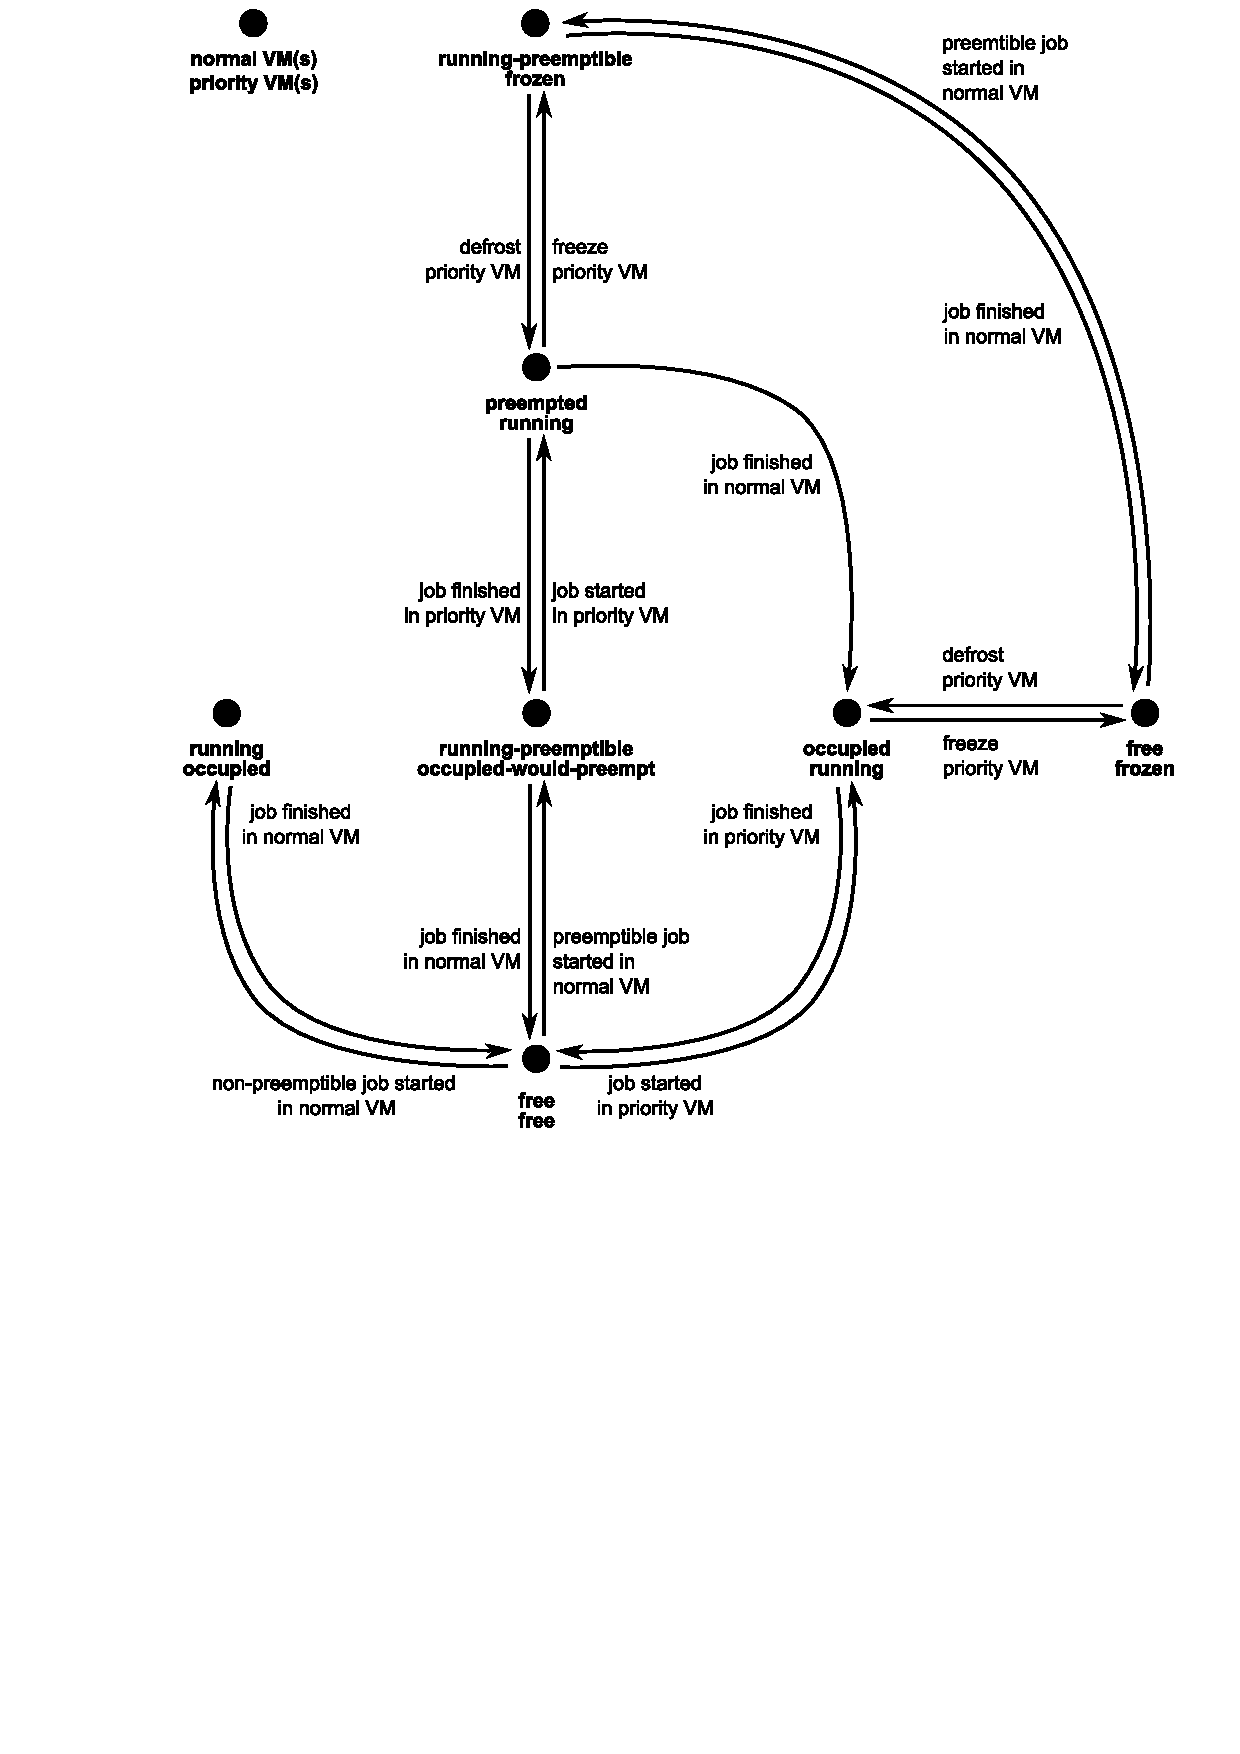
\includegraphics[clip=true,width=.97\linewidth,height=200mm]{frozen.pdf}
\end{wrapfigure}

\bigskip
\textbf{PBS scheduler} modified to:
\begin{itemize}
\item \rightskip=\z@skip respect Magrathea status -- submit only to domains
with Magrathea status \emph{free}, \emph{running},
\emph{occupied-would-preempt}, and \emph{running-preemptible}
\item \rightskip=\z@skip sort nodes using Magrathea status (non-preemption first)
\end{itemize}

\bigskip
\textbf{PBS server} modified to:
\begin{itemize}
\item \rightskip=\z@skip dedicate queue for high priority jobs
\item support frozen domains
\end{itemize}

\bigskip
\textbf{Job prologue/epilogue}:
\begin{itemize}
\item hooks to Magrathea
\item called on all nodes 
(for parallel jobs)
\end{itemize} 

\bigskip
\mypar Magrathea status also contains number of CPUs used by the virtual machine 
and \emph{length of preemption} -- number
of seconds jobs were preempted aggregated for each virtual node.

\mysectx{Ongoing work}
\mypar
Integration with a virtual cluster system for enabling seamless coexistence between virtual 
clusters and normal jobs and allowing a single scheduler to manage both entities at the 
same time to achieve better resource efficiency.

\mysectx{References}
\begin{thebibliography}{[1]}
\bibitem{VTDC}Miroslav Ruda and Ji\v{r}\'\i{} Denemark and Lud\v{e}k Matyska. 
Scheduling Virtual Grids: the Magrathea System. VTDC '07: 3rd
international workshop on Virtualization technology in distributed computing. 
Reno, USA, 2007.
\end{thebibliography}
\bigskip

\end{column}

\begin{column}{.45\linewidth}

\mysectx{Preemption}
\hrule height0pt
 Preemption techniques
{\begin{itemize}
 \item complete suspend (freezing)
 \item reducing memory and CPU
 \end{itemize}

\mypar 
Preemption overhead is critical for the second technique, especially for Xen.
While ballooning may be sufficient for simple jobs, it is incredibly slow for
intensive computations.

\mypar 
\alert{Kernel helper module} was created utilizing suspend-to-disk functions
for freeing memory which is than returned to Xen.

\mypar 
Test scenario: 14 parallel CPU and memory intensive processes consuming 15GB of
memory; preemption swaps out 14.7GB; processes are stopped using SIGSTOP before
reducing the memory.

\vspace*{-3ex} 
\renewcommand{\arraystretch}{1.2}
%\mybox{\begin{center}
\textbf{\large\begin{center}
\begin{tabular}{@{\ }l@{\quad}|@{\quad}r@{\ }l@{\ }}
disk speed & 2m & 50s\\
\hline
magrathea & 3m & 40s \\
\hline
balloon driver & 41m & 20s \\
\hline
w/o SIGSTOP &  \multicolumn{2}{r}{hours} \\
\end{tabular}\end{center}}
}

\mysectx{Conclusions}
{
\mypar 
Magrathea provides possibility to run different Linux flavors on one cluster node and
switch between them dynamically, gives us possibility to preempt
sequential jobs and therefore improves support for large
parallel jobs on our cluster, supports several active
domains concurrently on VServer, and allows for suspending jobs on Xen enabled
clusters.

\mypar 
Magrathea is deployed in production environment on computational nodes of
Meta{Center}, which provides a computational
infrastructure for various groups of users with specific requirements and its
resources are also provided for European grid infrastructure
EGEE.

\vspace*{1ex}
\hrule
This project has been supported by research intents ``Optical Network of
National Research and Its New Applications'' and ``Parallel and Distributed
Systems'' (M\v{S}M 6383917201, M\v{S}M 0021622419).
}

\end{column}
\end{columns}

%{\tiny This project has been supported by research intents ``Optical Network of
%National Research and Its New Applications'' and ``Parallel and Distributed
%Systems'' (M\v{S}M 6383917201, M\v{S}M 0021622419).}

\end{frame}

\end{document}
